\section{Graph DB}
Il grafo lo conosciamo, si ripresenta nella solita forma $G = (V,E)$, è infatti una collezione di nodi e archi. Diremo quindi che un grafo è un insieme di nodi e di relazioni fra loro, dove al suo interno i concetti più importanti, quelle che nel modello relazionale erano chiamate Entità, vengono ora modellate come nodi. Il nodo con cui le entità sono semanticamente associate si modellano come relazioni, tramite archi. \\
I grafi possono essere applicati in diversi ambiti:
\begin{itemize}
  \item social network
  \item sistemi di raccomandazione, che suggeriscono oggetti simili a utenti simili
  \item ambito geografico
  \item reti logistiche (per spedizione dei pachi ad esempio)
  \item transazioni finanziarie per la \textit{fraud detenction} (riconoscendo certi pattern sospetti, anche a livello geografico)
  \item master data management, rappresentazione unica della realtà
  \item bioinformatica
  \item controllo di autorizzazioni e accessi
\end{itemize}
Ci sono due modi per descrivere i dati, esistono :
\begin{itemize}
  \item \textbf{descrizione estensionale dei dati} quando si descrivono le istanze via-via, descrivendo anche istanze di tipo diverso (magari utenti e messaggi) usando la stessa sintassi del nodo (ugualmente per gli archi). La semantica viene data dall'etichetta
  \item \textbf{descrizione intensionale dei dati}, che bisognerebbe inferirla  direttamente dai dati e quindi non è applicabile
\end{itemize}


Nei RDBMS si ha il \textit{join} basato su valori, facendo uno \textit{scheme understanding} sulle varie tabelle, ottenendo quindi il risultato tramite anche più operazioni di \textit{join}. Si può avere però il problema applicativo, avendo magari \textbf{relazioni ad anello} tra le varie tabelle ad esempio una tabella persona che tramite una tabella amici ritorna su se stessa, avendo la tabella amici che esplode in numerosità. Si hanno potenzialmente livelli infiniti di \textit{join} si va incontro al \textbf{join bombing}, che fanno soffrire i DBMS. 

Notiamo che nei sistemi a grafo ora abbiamo gli archi, per collegare i nodi contenenti informazioni, mentre nei documentali avevamo identificatori che puntavano ad altri documenti: solitamente con un modello basato sui valori come se fossero \textit{foreign keys} dei RDBMS). Nei document based io devo definire un ordine gerarchico, devo fare un albero, e quinid i task di modellazione risultano molto complessi, con scarsa efficienza e complessità nel gestire dati fortemente connessi, mentre, con il referencing starei simulando una sorta di modello a grafo. \\

Un aspetto importante dei DB a grafo è che hanno forte potenza espressiva permettendo di caratterizzare i nodi con un certo \textit{tipo}, che possiamo chiamare etichette per caratterizzare il nodo, e definire le varie relazioni tramite archi.
\begin{figure}[H]
    \centering
    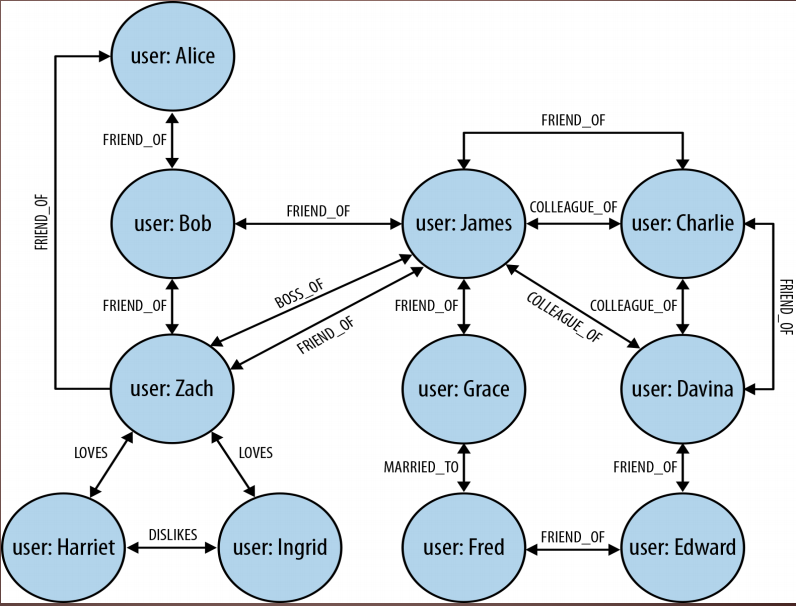
\includegraphics[scale = 0.4]{Immagini/slide-14-graphdb.PNG}
\end{figure}
Nei nodi posso rappresentare anche entità complesse, con vari attributi, ovvero varie \textbf{proprietà}. Ovviamente ogni nodo può avere un set di attributi diversi, avendo fortissima libertà di schema.\\
È un modello molto più immediato rispetto ad un RDBMS. Inoltre, nel caso si abbiano potenzialmente più relazioni tra due nodi basta contare quanti cammini orientati, che possono quindi passare per nodi intermedi diversi, esistono tra quei nodi per ottenere la cardinalità di tali relazioni. \\

Posso anche rappresentare un \textbf{property graph} in diversi modi:
\begin{itemize}
  \item quando sia nodi che relazioni possono avere proprietà espresse da chiave-valore, accettando quindi che i nodi abbiano un tipo
  \item altri ammettono array di valori
\end{itemize}
Si nota che invece in altri modelli NoSQL come RDF i nodi possono avere un tipo ma non proprietà e le relazioni non hanno proprietà, dovendo sempre rappresentare il tutto tramite triple \textbf{soggetto-predicato-oggetto}. \\
Il problema di modellazione dei grafi si ritrova quindi nella scelta di cosa mettere come nodo e cosa come relazioni (ed eventualmente le proprietà), avendo varie scelte modellistiche con vari pro e contro.\\ 
Anche nel caso dei GraphDB ogni vendor ha il suo linguaggio, anche se ne esiste uno \textit{standard}, chiamato \textbf{Gremlin}, che più che essere un linguaggio di interrogazione è un \textit{linguaggio di attraversamento dei grafi}. Questo tipo di linguaggio viene detto \textbf{vertex-based} che si usano per studiare la validità di predicati tramite l'attraversamento dei nodi.\\
\begin{enumerate}
  \item \textbf{graph processing}, dove ci si concentra sul processamento dei dati, processamento che viene eseguito tramite i grafi 
  \item \textbf{graph storage}, dove i dati vengono memorizzati in forma di grafo 
\end{enumerate}

In entrambi i casi la cosa può essere fatta in modo:
\begin{itemize}
  \item \textbf{nativo}:  \textit{native graph storage} per indicare che sono ottimizzati e progettati per le gestione stessa dei grafi. In questo caso comunque i dati vengono memorizzati in modo intelligente, memorizzando in modo vicino i nodi e il loro archi, facendo \textit{index free adjacency}, in modo che seguire gli archi uscenti da un nodo è molto più immediato.
  \item \textbf{non nativo}: \textit{non native graph storage} per indicare che i dati vengono trasformati da grafo ad un formato diverso tra cui relazionale, object oriented db. Si rischia comunque il \textit{join bombing}
\end{itemize}

Si hanno quindi due approcci principali per gestire un grafo:
\begin{itemize}
  \item \textbf{graph database}, ovvero un DBMS che gestisce in maniera persistente un grafo che viene usato per le transazioni. Si usa la dicitura OLTP
  \item \textbf{graph compute engine}, ovvero tecnologie per l'analisi \textit{off line} dei grafi. Si usa la dicitura OLTP
\end{itemize}

I graph database supportano le operazioni CRUD (come tutti i modelli NoSQL): \textbf{C}reate, \textbf{R}ead, \textbf{U}pdate e \textbf{D}elete.

Come abbiamo visto si studiano gli attraversamenti del grafo per fare le query in modo performante non facendo join ma attraversando e basta. Sono inoltre costruiti per essere usati nei sistemi transazionali (OLTP), per dati compessi e connessi. \\ 

Abbiamo detto che per i sistemi nativi sono ottimizzati per i grafi e vengono poi discussi in seguito. Ci sono poi i grafici non nativi che trasformano i dati in un grafo relazionale object oriented. 
Si ha un problema grave coi grafi: \textbf{i grafi non scalano bene e non possono essere facilmente frammentati}.\\ Partizionare un grafo raramente è possibile, in quanto comporta un taglio di relazioni. Se quindi si vuole scalare bisogna passare, alla fine, ad un altro modello, aggiungendo però costo di comunicazione tra il modello a grafo e il nuovo modello scelto, aggiungendo un layer software.\\

Il sistema fondamentale dei \textbf{native graph storage} memorizzano in modo vicino i nodi e il loro archi, facendo \textit{index free adjacency}, in modo che seguire gli archi uscenti da un nodo è molto più immediato.

\subsection{Neo4j}
Abbiamo già introdotto precedentemente Neo4j. Sappiamo che è nativo sia per il \textit{graph processing} che per il \textit{graph storage} .\\

Approfondiamo quindi il \textbf{linguaggio di interrogazione di Neo4j}, chiamato \textbf{Cypher} (\textit{OpenCypher} nella versione open).\\ 
Cypher è definito come un \textbf{pattern-matching query language}. È un linguaggio simil-umano, espressivo, dichiarativo (si dice il cosa e non il come), che consente operazioni di aggregazione, sorting e di limit e permette di aggiornare il grafo.\\ Un formato in modo testuale viene rappresentato con le parentesi tonde per i nodi e le quadre per gli archi. Le relazioni orientate vengono indicate tramite $->$ o $<-$.
Per esempio \\ $(c)-[:KNOWS]->(b)-[:KNOWS]->(a), (c)-[:KNOWS]->(a)$, possiamo rappresentare in questo modo una lista di amici. \\ Con la virgola $,$ andiamo a rappresentare una $\land$. Un modo equivalente di rappresentazione della stessa query :\\
$(c)-[:KNOWS]->(b)-[:KNOWS]->(a)<-(c)-[:KNOWS]$
Vediamo quindi un'interrogazione classica in Cypher, dove si cercano tutti gli utenti tali per cui conosce qualcuno $a$ che conosce qualcuno $b$ e che sono etichettati come \textbf{Michael}, ritornando $a$ e $b$: 
\begin{lstlisting}
    MATCH(c:user)
    WHERE (c)-[:KNOWS]->(b)-[:KNOWS]->(a),
          (c)-[:KNOWS]->(a), c.user="Michael"
    RETURN a, b
\end{lstlisting}
Il risultato sarà una \textbf{tabella} che contiene tutte le coppie $a$ e $b$. Avrà dei dati ridondati a causa della dualità intrinseca di avere $a$ che conosce $b$, cosa che probabilmente porta ad avere che $b$ conosce $a$. \\
Quindi il risultato \textbf{non sempre} è un grafo (mentre nel documentale era sempre un documento e nel relazionale una tabella) ma può anche essere altro, ad esempio una tabella. Non è quindi sempre possibile concatenare query in quanto potrei non avere un grafo in uscita.\\
Si hanno delle clausole nel linguaggio Cypher:
\begin{lstlisting}
    WHERE 'per imporre criteri di filtraggio tramite pattern-matching dei risultati'
    CREATE / CREATE UNIQUE 'per creare nodi e relazioni'
    DELETE 'per cancellare nodi, relazioni e propriet\textnormala'
    SET 'per impostare dei valori alle proprieta'
    FOREACH 'per fare un update per elementi del grafo posti in una lista '
    UNION 'per unire i risultati + query'
    WITH 'per concatenare query propagando i risultati in pipe'
\end{lstlisting}


\textbf{Qui fa un esempio che personalmente poco mi interessa cosa? inutile}

Abbiamo già visto che non ha meccanismi nativi di frammentazione, avendo scelto di sfruttare la \textit{index free adjacency} e la modellazione a grafo, non permettendo scalabilità. In compenso garantisce però
\begin{itemize}
  \item permette le transazioni con tutte le proprietà ACID, con meccanismi di locking
  \item garantisce la recoverability
  \item garantisce la disponibilità
  \item garantisce la scalabilità, infatti nonostante le limitazioni, garantisce l'\textbf{alta disponibilità}.
\end{itemize}
Per la scalabilità l'idea è che è possibile andare a definire un cluster di nodi Neo4j, alcuni chiamati \textbf{core server}, ovvero nodi per cui tutte le scritture sono fatte in contemporanea, essendo quindi sincronizzati. Si hanno poi gli altri nodi che sono chiamati \textbf{replica server}, che sono di sola lettura e vengono anche usati per reporting analysis etc$\ldots$. Fatta una query essa comunque non viene distribuita ma eseguita sul nodo più vicino. Tutto questo sistema è detto \textbf{casual clustering}.\\ 
Si ha una bassa \textbf{latenza} nelle query in quanto si usa un indice per risalire al primo nodo e poi si procede coi cammini, avendo quindi che le performances non dipendono dalla grandezza del dataset ma solo da quali sono i dati richiesti dalla query.\\

In situazioni reali, ad esempio un e-commerce, posso avere i dati salvati in vari DBMS, sia relazionali che NoSQL, a seconda dei dati che contengono. Dover gestire tutti questi modelli diversi è molto complicato, ma sensato in base al tipo di dati. Ho quindi una sorta di \textbf{mondo poliglotta}. 
\subsection{ArangoDB}
In questo mondo poliglotta complesso ci arriva in soccorso un particolare DBMS: \textbf{ArangoDB}.\\ 
Il DBA dovrebbe conoscere tutti i modelli in uso e tutti i linguaggi associati, essendo anche in grado di gestire i vari conflitti. ArangoDB introduce il concetto di \textbf{db poliglotta}, supportando i modelli: \textbf{chiave-valore}, \textbf{document based}, \textbf{graph db} e \textbf{ricerca full text}.

Rispetto ai modelli a grafo con storage non nativo il linguaggio di query di ArangoDB, chiamato \textbf{AQL (\textit{Arango Query language})}, garantisce la possibilità di interrogare dati in formato: json quindi in maniera documentale, a grafo, in formato key-value o  usando full text search. \\

\textbf{Avviso: non si è soffermato è roba accenata ma non nel dettaglio}
Ad alto livello Arango organizza i dati in database e collezioni, dove le collezioni memorizzano documenti o similari. I documenti, come già accennato, sono documenti json annidati.\\
\textbf{Qui inoltre fa solamente un esempio, anche questo non credo serva}\\
Possiamo comunque interrogare usando il modello a grafo e tali query mostrano quali documenti sono collegati (direttamente o indirettamente) ad altri documenti, specificando il cammino per ottenere il collegamento. Queste connessioni tra documenti sono chiamate \textbf{edges} che sono salvati in edge collections. Gli \textit{edges} hanno sempre due attributi che si riferiscono ai nodi entranti e uscenti: $_from $ e $_to$.

Si hanno vari metodi di scalabilità, avendo le modalità di deploy: a singola istanza, master/slave, active failover, cluster e multiple datacenters.

\subsection{Active Failover}
Nel modello master/slave quando il master fallisce lo slave non può essere sostituito e quindi si è pensato al modello \textbf{active failover}. 
In questo modello esistono delle istanze \textit{single-server} chiamate \textbf{leader} che sono in lettura e scrittura, ed esistono delle istanze, sempre \textit{single-server}, chiamate \textbf{followers} che non sono altro che vecchi slave passivi e non scrivibili.
Il leader invia le operazioni di scrittura ai followers che replicano in modo asincrono i dati tramite la cosiddetta \textbf{Write-Ahead Log (\textit{WAL})}, ovvero il leader prima salva su un file di log e poi sul disco. Il file di log, tramite replica incrementale viene aggiornato. \\
Esiste poi almeno un \textbf{agency} che controlla le configurazioni dei leader e dei followers e controlla che siano tutti disponibili. Qualora l'agency si accorgesse che un server leader non è più disponibile promuove, con un meccanismo elettivo, un follower a leader. Resta quindi una sorta di master/slave ma con gli agency che procedono con il controllo e la rielezione.

\subsection{Cluster}
Il cluster è un'evoluzione del Active Failover, avendo più \textbf{coordinator} che si connettono con i client. I coordinator effettuando le query e gli \textbf{agency} non si occupano di altro che: dell'elezione del leader nel caso in cui un coordinator fallisce e della sincronizzazione dei dati per l'intero cluster. 
Si hanno poi i \textbf{DB server}, di tipo slave, che in caso di fallimento non comporta problemi in quanto l'agency attua le solite politiche di aumento repliche, bilanciando nuovamente i dati in caso di sharding.\\ 

Lo sharding avviene in partizioni da almeno 40gb, con un meccanismo simile a quello di MongoDB: ogni server avrà associato uno shard, e ogni server avrà le repliche di altri server. \\
Si hanno due soluzioni per la scrittura: 
\begin{enumerate} 
    \item il protocollo \textbf{read once write all (ROWA)} che obbliga il coordinator a scrivere su tutte le repliche 
    \item il coordinatore scrive solo dove si ha la copia primaria e poi si hanno le repliche, è la soluzione \textbf{oneshard} (che era chiamato \textbf{write concern} in MongoDB) 
\end{enumerate}

\subsection{Cluser to Cluster}
Una soluzione asincrona di tipo \textbf{one way} in cui prendo un cluster e lo copio interamente in un altro, usando una coda come \textbf{kafka}. La replica è one way per cui scarico dal primary alla replica o viceversa in tempi diversi, non contemporaneamente. Non è pensato per fare una replica del single-server (userei il master/slave).
